% !TeX root = ../main.tex
\chapter{训练}\label{ch3}

如 \ref{sec1.1} 节所述,训练模型包括最小化损失 $\mathcal{L}(w)$,它反映了预测器 $f(\cdot;w)$ 在\keyterm{训练集} $\mathcal{D}$ 上的表现。

由于模型通常非常复杂,并且其表现与损失最小化程度直接相关,因此这里的最小化是一个关键挑战,涉及计算和数学难题。

\section{损失}\label{sec3.1}

公式 \ref{eq1.1} 中的\keyterm{均方误差}示例是用于预测连续值的标准损失。

在密度建模中,标准损失是数据的似然度。如果 $f(x;w)$ 被解释为归一化的对数概率或对数密度,那么损失就是其值在训练样本上的总和的相反数,这对应于数据集的似然度。

\subsubsection*{交叉熵}

对于\keyterm{分类},通常的策略是模型的输出是一个向量,其中每个类别 $y$ 对应一个分量 $f(x;w)_y$,这被解释为非归一化概率的对数或 \keyterm{logit}。

如果 $X$ 为输入信号,$Y$ 为要预测的类别,我们可以根据 $f$ 计算\keyterm{后验概率}估计:
\[\hat{P}(Y=y \mid X=x) = \frac{\exp f(x;w)_y}{\sum_{z}\exp f(x;w)_z}\]
该表达式通常称为 logits 的 \keyterm{softmax},或更准确地说,称为 \keyterm{softargmax}。

为了与这种解释保持一致,模型应该被训练来最大化真实类别的概率,因此要最小化交叉熵,其表达式如下:
\begin{align*}
    \mathcal{L}_{ce}(w) &= -\frac{1}{N}\sum_{n=1}^{N} \log \hat{P}(Y=y_n \mid X=x_n) \\
    &= \frac{1}{N}\sum_{n=1}^{N} \underbrace{-\log \frac{\exp f(x_n;w)_{y_n}}{\sum_{z}\exp f(x_n;w)_z}}_{L_{ce}(f(x_n;w),y_n)}
\end{align*}

\subsubsection*{对比损失}

在某些设置中,即使要预测的值是连续的,监督也会采取排名约束的形式。这种情况的典型领域是\keyterm{度量学习},其目标是学习样本之间距离的度量,使得来自某个语义类别的样本 $x_a$ 与同一类别中的任意样本 $x_b$ 之间的距离都比来自另一个类别的任意样本 $x_c$ 之间的距离更近。例如,$x_a$ 和 $x_b$ 可以是某个人的两张照片,而 $x_c$ 则是另一个人的照片。

这种情况的标准方法是最小化\keyterm{对比损失},在这种情况下,例如,三元组 $(x_a,x_b,x_c)$,满足 $y_a = y_b \ne y_c$,求和
\[\max(0,1-f(x_a,x_c;w)+f(x_a,x_b;w))\]
除非 $f(x_a,x_c;w) \ge 1+f(x_a,x_b;w)$,否则该量将严格为正。

\subsubsection*{工程化损失}

通常,在训练期间最小化的损失并不是最终想要优化的实际量,而是一个代理量,是为了让找到最佳模型参数更为容易。例如,尽管实际的性能度量是分类错误率,但交叉熵是分类的标准损失,因为后者没有提供信息梯度,这是我们将在 \ref{sec3.3} 节中看到的关键要求。

还可以在损失中添加取决于模型本身的可训练参数项,以支持某些配置。

例如,\keyterm{权重衰减}正则化包括向损失中增加一个与参数平方和成比例的项。这可以被解释为在参数上施加了一个高斯贝叶斯先验,它偏好较小的值,从而减少了数据的影响。这会降低其在训练集上的表现,但会减少训练表现与新的、未见过的数据上的表现之间的差距。

\section{自回归模型}\label{sec3.2}

自回归模型是一类关键方法,特别适用于处理自然语言处理和计算机视觉中的离散序列。

\subsubsection*{概率的链式法则}

这些模型使用概率论中的\keyterm{链式法则}:
\begin{align*}
    P(&X_1 = x_1,X_2 = x_2,\dots,X_T = x_T) = \\
    &P(X_1 = x_1) \\
    \times &P(X_2 = x_2 \mid X_1 = x_1) \\
    &\dots \\
    \times &P(X_T = x_T \mid X_1 = x_1,\dots,X_{T-1} = x_{T-1})
\end{align*}
尽管这种分解对于任何类型的随机序列都有效,但当感兴趣的信号是来自有限\keyterm{词汇表} $\{1, \dots ,K\}$ 的 \keyterm{Token} 序列时,它特别有效。

按照约定,附加 Token $\emptyset$ 代表``未知''量,我们可以将事件 ${X_1 = x_1,\dots,X_t = x_t}$ 表示为向量 $(x_1,\dots,x_t,\emptyset,\dots,\emptyset)$。则模型
\[f : \{\emptyset,1,\dots,K\}^T \to \mathbb{R}^K\]
在给定这样的输入的情况下计算与
\[\hat{P}(X_t \mid X_1 = x_1,\dots,X_{t-1} = x_{t-1})\]
相对应的 $K$ 个 \keyterm{logits} 的向量 $l_t$,允许在给定先前 Token 的情况下对一个 Token 进行采样。

链式法则确保在给定先前采样的 $x_1,\dots,x_{t-1}$ 的情况下,通过一次次地对第 $T$ 个 Token $x_t$ 进行采样,我们能够得到一个遵循联合分布的序列。这是一个\keyterm{自回归}生成模型。

训练这样的模型可以通过最小化训练序列和时间帧上的\keyterm{交叉熵损失}
\[Lce\big(f(x_1,\dots,x_{t-1},\emptyset,\dots,\emptyset;w),x_t\big)\]
之和来完成,这在形式上等同于最大化真实 $x_t$ 的似然。

传统上监测的值不是交叉熵本身,而是\keyterm[困惑度]{困惑度(Perplexity)},其定义为交叉熵的指数。它对应于具有相同熵的均匀分布的值的数量,这通常更易于解释。

\subsubsection*{因果模型}

我们所描述的训练过程对于每个 $t$ 都需要不同的输入,而且在 $t < t'$ 的情况下所做的大部分计算会在 $t'$ 时重复进行。这是极其低效的,因为 $T$ 通常是几百或几千的数量级。

解决这个问题的标准策略是设计一个模型 $f$ 一次性预测所有 logits 向量 $l_1,\dots,l_T$,即:
\[f : {1,\dots,K}^T \to \mathbb{R}^{T \times K}\]
但存在计算结构使得计算 $x_t$ 的 logits $l_t$ 仅依赖于输入值 $x_1,\dots,x_{t-1}$。

\begin{figure}
    \centering
    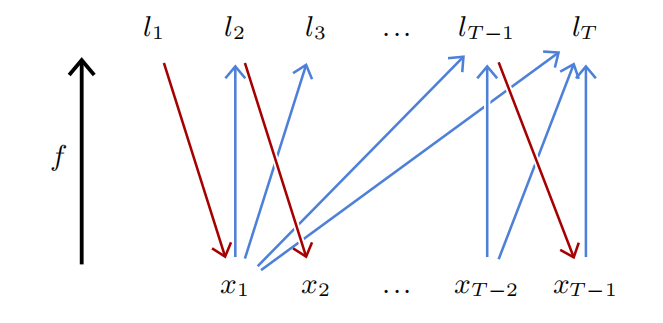
\includegraphics[width=0.9\textwidth]{fig/fig3.1.png}
    \caption[因果自回归模型]{如果输入序列的一个时间帧 $x_t$ 调节预测的 logits $l_s$ 只在 $s > t$ 时才有效,如蓝色箭头所示,则自回归模型 $f$ 是因果模型。这允许在训练期间一次性计算所有时间帧的分布。然而,在采样过程中,$l_t$ 和 $x_t$ 是顺序计算的,后者是用前者采样的,如红色箭头所示。}
    \label{fig3.1}
\end{figure}

这样的模型称为\keyterm{因果模型},因为在时间序列的情况下,它对应于不让未来影响过去,如图 \ref{fig3.1} 所示。

其结果是,每个位置上的输出都假设输入只在该位置之前可用的情况下所得到的。在训练过程中,这使得我们能够计算一个完整序列的输出,并最大化该序列所有 token 的预测概率,这又归结为最小化每个 token 的交叉熵之和。

请注意,为了简单起见,我们将 $f$ 定义为对长度固定为 $T$ 的序列进行操作。然而,实际使用的模型,例如我们将在 \ref{sec5.3} 节中看到的 Transformer 模型,能够处理任意长度的序列。

\subsubsection*{分词器(Tokenizer)}

处理自然语言时,一个重要技术细节是,token 的表示方法多种多样,从最细粒度的单个符号到整个单词,不一而足。而 token 表示的转换是由一个称为\keyterm{分词器}(\keyterm{tokenizer})的独立算法来完成的。

一种标准的方法是\keyterm{字节对编码}(\keyterm{Byte Pair Encoding},\keyterm{BPE}) \citep{srivastava14a},它通过分层合并字符组来构造 token,尝试获取代表不同长度但频率相似的单词片段的 token,并将 token 分配给长的高频片段以及罕见的单个符号。

\section{梯度下降}\label{sec3.3}

除了在 \ref{sec1.2} 节中看到的线性回归等特定情况外,最优参数 $w^*$ 没有闭合形式的表达式。在一般情况下,最小化函数的选择工具是\keyterm{梯度下降}。它首先使用随机值 $w_0$ 初始化参数,然后通过迭代\keyterm{梯度步骤}来改进该估计,每个梯度步骤包括计算损失相对于参数的梯度,并减去其中的一小部分:
\begin{equation}
    w_{n+1} = w_n - \eta \nabla \mathcal{L}_{\mid w}(w_n)\label{eq3.1}
\end{equation}
此过程相当于将当前估计值超微朝局部最优方向最大化地减小 $\mathcal{L}(w)$,如图 \ref{fig3.2} 所示。

\begin{figure}
    \centering
    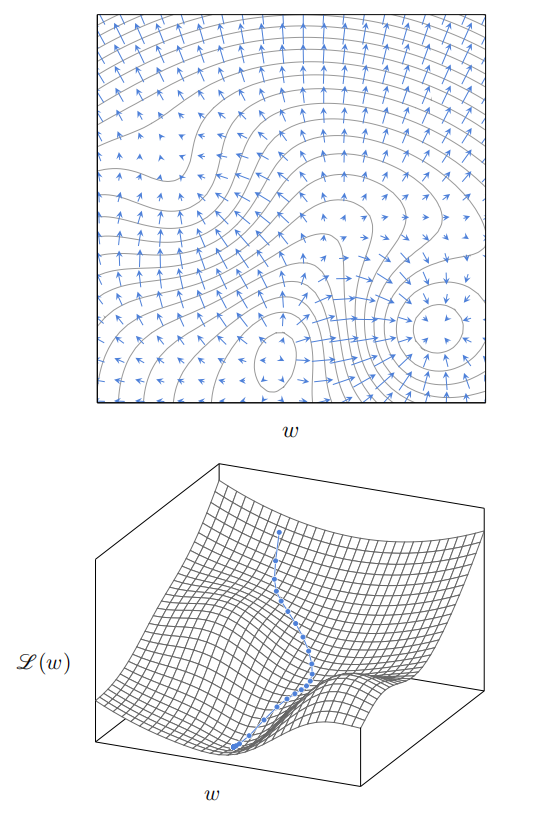
\includegraphics[width=0.9\textwidth]{fig/fig3.2.png}
    \caption[梯度下降]{对于每个点 $w$,梯度 $\nabla \mathcal{L}_{\mid w}(w)$ 都处于使 $\mathcal{L}$ 增加最大化的方向,与水平曲线(上图)正交。梯度下降通过在每一步减去梯度的一小部分来迭代地最小化 $\mathcal{L}(w)$,从而产生遵循最陡下降的轨迹(下图)。}
    \label{fig3.2}
\end{figure}

\subsubsection*{学习率}

\keyterm{元参数} $\eta$ 称为\keyterm{学习率}。它是一个正值,可调节最小化完成的速度,必须谨慎选择。

如果该值太小,优化会很慢,并可能会过早陷入局部最小值。如果该值太大,优化可能会在某个最小值附近反复跳动,从而永远无法下降到该最小值。正如我们将在 \ref{sec3.6} 节中看到的,学习率可以依据迭代次数 $n$ 来调节。

\subsubsection*{随机梯度下降}

实际中使用的所有损失都可以表示为每一小组样本或每个样本的平均损失,例如:
\[\mathcal{L}(w) = \frac{1}{N} \sum_{n=1}^{N} \mathcal{l}_n(w)\]
其中对于某个 $L$,$\mathcal{l}_n(w) = L(f(x_n;w),yn) f$,那么梯度可以表示为
\begin{equation}
    \nabla \mathcal{L}_{\mid w}(w) = \frac{1}{N} \sum_{n=1}^{N} \nabla \mathcal{l}_{n \mid w}(w)\label{eq3.2}
\end{equation}
尽管通常来说这里地计算量很大,由此产生的\keyterm{梯度下降}将精确计算公式 \ref{eq3.2} 中的求和,然后根据公式 \ref{eq3.1} 更新参数。然而,在合理的可交换性假设下,例如,如果样本已被适当地随机打乱,则方程 \ref{eq3.2} 的任何部分之和都是总和的无偏估计,尽管这样做会带来噪声。因此,从部分之和更新参数相当于在相同计算预算下执行更多的梯度步骤,并且梯度估计的噪声更大。由于数据的冗余,这恰好是一种更有效的策略。

我们在 \ref{sec2.1} 节中看到,处理一批大小适合计算设备内存的样本通常与处理单个样本一样快。因此,标准方法是将全集 $\mathcal{D}$ 分成\keyterm{批次},并根据每个批次计算的梯度估计来更新参数。这称为小批次随机梯度下降,简称\keyterm{随机梯度下降}(\keyterm{SGD})。

需要注意的是,这一过程是极其缓慢的,小批次数据和梯度步骤的数量通常达到数百万的量级。

与许多算法一样,直觉在高维中会崩溃,尽管看起来这个过程很容易陷入局部最小值,但实际上,由于参数数量、模型设计和数据的随机性,其效率远远高于人们的预期。

人们已经提出了许多该标准策略的变体。其中最流行的是 \citep{arxiv-1412.6980},它可以进一步对每个梯度分量的平均值和方差进行估算,并自动将其归一化,避免了缩放问题以及模型不同部分训练速度不一致问题。

\section{反向传播}\label{sec3.4}

使用\keyterm{梯度下降}需要一种技术手段来计算 $\nabla \mathcal{l}_{\mid w}(w)$,其中 $\mathcal{l} = L(f(x;w);y)$。鉴于 $f$ 和 $L$ 都是标准张量运算的组合,对于任意数学表达式,微分\keyterm{链式法则}都可以得到它的表达式。

为了使符号表示更加简洁,我们不会特别指明梯度计算的具体位置,因为上下文已经清楚地说明了这一点。

\begin{figure}
    \centering
    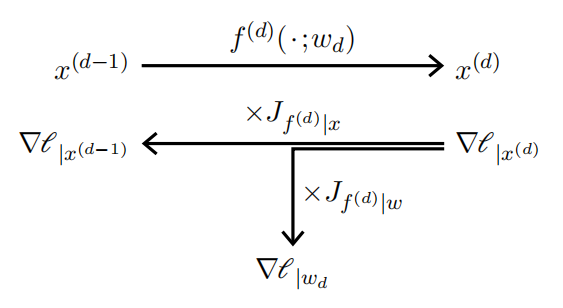
\includegraphics[width=0.9\textwidth]{fig/fig3.3.png}
    \caption[反向传播]{给定模型 $f = f^{(D)} \circ \dots \circ f^{(1)}$,正向传递(上图)包括按顺序计算映射 $f^{(d)}$ 的输出 $x^{(d)}$。反向传递(下图)通过将它们乘以雅可比行列式来计算相对于激活 $x^{(d)}$ 和参数 $w_d$ 的损失梯度。}
    \label{fig3.3}
\end{figure}

\subsubsection*{正向和反向传递}

考虑映射组合的一个简单情形:
\[f = f^{(D)} \circ f^{(D-1)} \circ \dots \circ f^{(1)}\]
$f(x;w)$ 的输出可以从 $x^{(0)} = x$ 开始并通过迭代应用
\[x^{(d)} = f^{(d)}\Big(x^{(d-1)};wd\Big)\]
来计算,以 $x^{(D)}$ 为终值。

这些中间结果 $x^{(d)}$ 的各个标量值传统上称为\keyterm{激活},名字参考了神经元的激活,值 $D$ 是模型的\keyterm{深度},各个映射 $f(d)$ 被称为\keyterm{层},正如我们将在 \ref{sec4.1} 节中看到的,它们的顺序评估是正向传递(参见上面的图 \ref{fig3.3})。

相反,损失相对于 $f^{(d-1)}$ 的输出 $x^(d-1)$ 的梯度 $\nabla \mathcal{l}_{\mid x}(d-1)$ 是梯度 $\nabla \mathcal{l}_{\mid x}(d)$ 相对于 $f(d)$ 的输出乘以 $f(d-1)$ 相对于其变量 $x$ 的雅可比行列式 $J_{f^{(d-1)} \mid x}$。因此,所有 $f(d)$ 的输出的梯度可以从 $\nabla \mathcal{l}_{\mid x^{(D)}} = \nabla L_{\mid x}$ 开始向后递归计算。

我们在训练中关注的梯度,即 $\nabla \mathcal{l}_{\mid w_d}$,是相对于 $f(d)$ 输出的梯度乘以 $f(d)$ 相对于参数的雅可比矩阵 $J_{f^{(d)} \mid w}$。

这种针对中间激活梯度的迭代计算,与针对层参数梯度的迭代计算相结合,就是\keyterm{反向传递}(见图 \ref{fig3.3} 的下半部分)。这种计算与梯度下降过程的结合称为\keyterm{反向传播}。

实际上,正向和后向传递的实现细节对程序员是隐蔽的。深度学习框架能够自动构建计算梯度的操作序列。

\keyterm{Autograd} \citep{arxiv-1502.05767} 是一种特别方便的算法,它追踪张量运算并动态构建梯度运算符组合。得益于此,操作张量的命令式编程可以自动计算任意量相对于任意其他量的梯度。

\subsubsection*{资源利用}

就\keyterm{计算成本}而言,如我们将要看到的,大部分计算量投入到了线性运算中,每个运算在正向传递中需要一个矩阵乘积,在反向传递中需要两个与雅可比矩阵相关的乘积运算,这使得反向传递的成本大约是正向传递的两倍。

在推理过程中,\keyterm{内存需求}大致相当于最占资源的单个层所需的内存。然而,对于训练来说,反向传递需要保留在正向传递中计算出的激活值,以便计算雅可比矩阵,这导致内存使用量与模型的深度成正比增长。存在一些技术可以通过依赖\keyterm{可逆层} \citep{arxiv-1707.04585} 或使用\keyterm{检查点}来交换内存使用与计算量,检查点包括只存储某些层的激活值,并在反向传递过程中通过部分正向传递动态地重新计算其他层 \citep{arxiv-1604.06174}。

\subsubsection*{梯度消失}

在训练大型网络时,一个关键的历史问题是,当梯度通过某个运算符反向传播时,可能会被一个乘法因子缩放,因此当它穿过许多层时,梯度可能会呈指数级减小或增大。防止梯度爆炸的标准方法是\keyterm{梯度范数裁剪},如果梯度的范数超过了阈值,就重新缩放梯度,使其范数达到一个固定的阈值 \citep{pascanu13}。

当梯度呈指数下降时,被称为\keyterm{梯度消失},它可能使训练变得不可能进行,或者以较温和的形式,导致模型的不同部分以不同的速度更新,从而降低它们之间的共适性 \citep{glorot10a}。

正如我们将在第 \ref{ch4} 章中看到的,为了防止这种情况发生,人们已经开发出多种技术,这反映出对深度学习成功至关重要的视角变化:人们不再试图改进通用的优化方法,而是转而致力于工程化模型本身,使其更易于优化。

\section{深度值}\label{sec3.5}

正如``深度学习''这一术语所示,有用的模型通常是一长串映射的组合。通过\keyterm{梯度下降}来训练这些模型,即便这一过程是渐进且局部的,也会导致映射关系之间发生复杂的共适性。

我们可以用一个简单的 $\mathbb{R}^2 \to \mathbb{R}^2$ 模型来说明这种行为,该模型组合了八层,每层将其输入乘以 $2 \times 2$ 矩阵,并对每个部分应用 Tanh,最后是一个线性分类器。这是我们将在 \ref{sec5.1} 节中看到的标准\keyterm{多层感知机}的简化版本。

如果我们在简单二元分类任务上使用\keyterm{随机梯度下降}(\keyterm{SGD})和\keyterm{交叉熵}训练该模型(如图 \ref{fig3.4},左上部分),矩阵会发生共适应使空间变形,直到分类正确,这意味着数据在最终仿射操作之前已线性可分(如图 \ref{fig3.4},右下部分)。

\begin{figure}
    \centering
    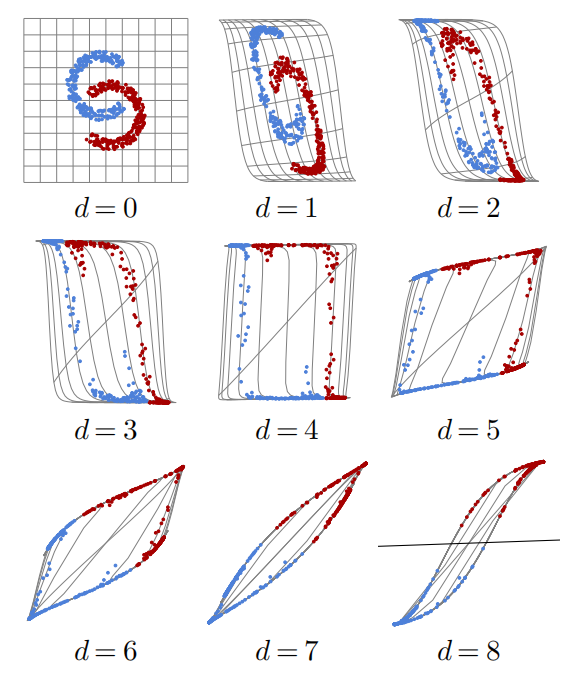
\includegraphics[width=0.9\textwidth]{fig/fig3.4.png}
    \caption[特征扭曲]{从模型本身的输入(左上角)开始,每个图显示了空间的变形以及经过 $d$ 层处理后 $\mathbb{R}^2$ 中训练点的最终位置。最后一张图(右下角)中的斜线显示了最终的仿射决策。}
    \label{fig3.4}
\end{figure}

这样的例子让我们一睹深度模型可以实现的目标;然而,由于要处理的信号和内部表征的维度都很低,因此它在一定程度上具有误导性。 为了便于可视化,这里所有内容都保持为二维,而真实模型则利用高维表征,特别是通过提供多个自由度来促进优化。

二十年来积累的经验证据表明,在各个应用领域实现最先进的性能需要具有数十层的模型,比如\keyterm{残差网络}(详见 \ref{sec5.2} 节)或 \keyterm{Transformer}(详见 \ref{sec5.3} 节)。

理论结果表明,对于固定计算预算或参数数量,增加深度会导致生成的映射更加复杂 \citep{1602.04485}。

\section{训练协议}\label{sec3.6}

训练深度网络需要定义一个协议来充分利用算力和数据,并确保模型在新数据上的表现良好。

正如我们在 \ref{sec1.3} 节中看到的,仅凭训练样本上的表现可能会产生误导,因此在最简单的设置中,至少需要两组样本:一组是\keyterm{训练集},用于优化模型参数,另一组是\keyterm{测试集},用于评估训练好的模型的表现。

此外,通常还有一些\keyterm{元参数}需要调整,特别是那些与模型架构、学习率和损失中的正则化项相关的参数。在这种情况下,需要一个与训练集和测试集都不相交的\keyterm{验证集}来评估最佳配置。

完整的训练通常被分解为若干个轮次(\keyterm{epoch}),每个轮次对应于将所有训练样本进行一次遍历。损失的常见动态是,只要优化过程在运行,训练损失就会降低,而验证损失可能在一定数量的轮次后达到最小值,然后开始增加,这反映了\keyterm{过拟合}情况,正如 \ref{sec1.3} 中介绍的那样,如图 \ref{fig3.5} 所示。

\begin{figure}
    \centering
    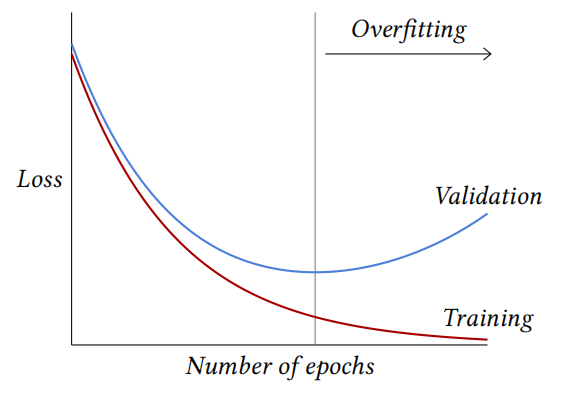
\includegraphics[width=0.9\textwidth]{fig/fig3.5.png}
    \caption[训练损失和验证损失]{随着训练的进行,通常通过损失来监控模型的性能。训练损失是推动优化过程的动力,它会逐渐减少,而验证损失则是基于另一组样本估计的,用以评估模型的过拟合情况。当模型开始考虑到特定于当前训练集的随机结构时,就会出现过拟合,导致验证损失开始增加。}
    \label{fig3.5}
\end{figure}

矛盾的是,尽管大型模型由于其能力强大,理应受到严重的过拟合影响,但随着训练的进行,它们通常会持续改进。这可能是因为当模型在训练集上的表现接近完美时,模型的\keyterm{归纳偏差}成为优化的主要驱动力 \citep{arxiv-1812.11118}。

一个重要的设计选择是训练期间的\keyterm{学习率安排},即每次梯度下降迭代中\keyterm{学习率}的具体值。一般的策略是,学习率初始应设置得较大,以避免优化过程过早地陷入不良的局部最小值中;过程中学习率应该逐渐变小,从而使得优化后的参数值不会在损失曲线的狭窄山谷中反弹,而是能够达到一个良好的最小值。

极大模型的训练可能需要在数千个强大的 GPU 上训练数月之久,耗资数百万美金。在这个规模上,训练可能涉及许多人工干预,特别是根据损失演变的动态来给与指导。

\section{规模的好处}\label{sec3.7}

大量经验结果表明,只要模型大小相应增大,根据著名的\keyterm{规模定律}(\keyterm{scaling law}),性能(例如测试数据上的损失估计)就会随着数据量的增加而提高 \citep{arxiv-2001.08361}(见图 \ref{fig3.6})。

\begin{figure}
    \centering
    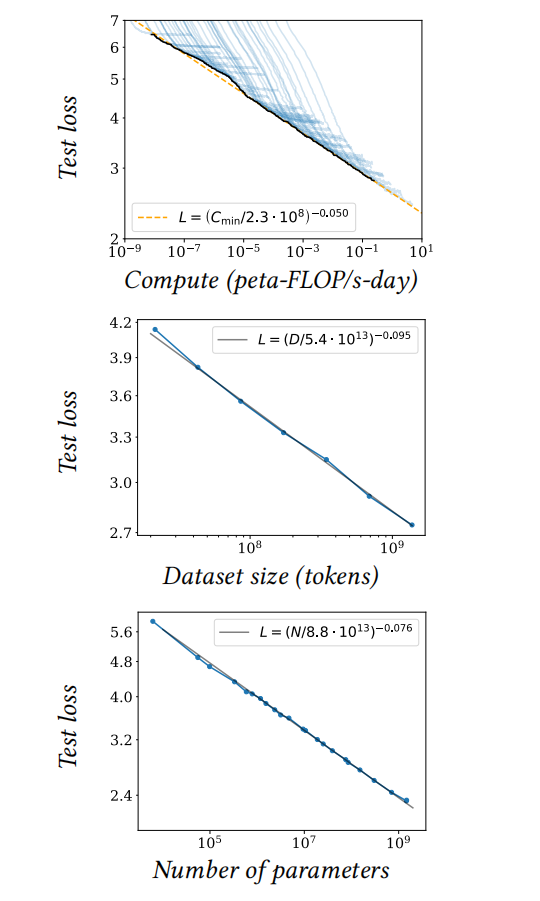
\includegraphics[width=0.9\textwidth]{fig/fig3.6.png}
    \caption[规模定律]{语言模型的测试损失与计算量(以 petaflop/s-day 计)、数据集大小(以 tokens 计)以及模型大小(以参数量计)之间的关系 \citep{arxiv-2001.08361}。}
    \label{fig3.6}
\end{figure}

在数十亿样本规模下,从规模定律中受益是可能的,部分原因在于模型的结构可塑性,正如我们将会看到的,这使得我们可以通过增加层数或特征维度来任意扩大模型规模。但也可以通过模型和\keyterm{随机梯度下降}实现的分布式计算特性来实现,这种做法一次只需要极少一部分数据,并且能够处理的数据量比计算设备内存大好几个数量级的数据集。这导致了模型的指数级增长(如图 \ref{fig3.7} 所示)。

\begin{figure}
    \centering
    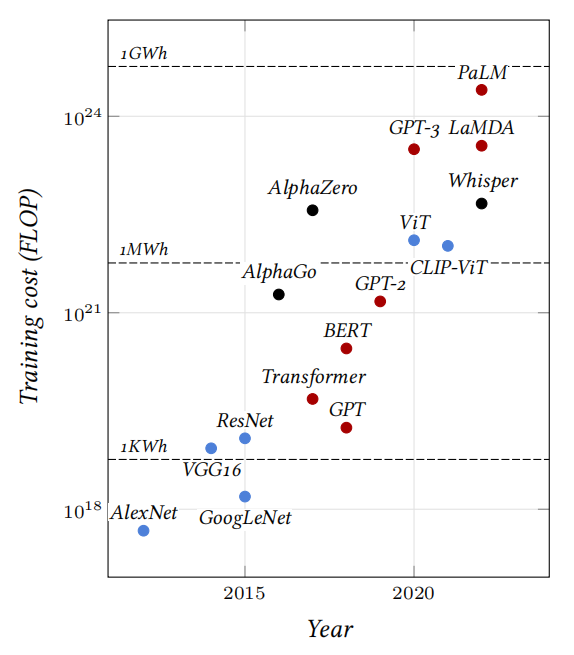
\includegraphics[width=0.9\textwidth]{fig/fig3.7.png}
    \caption[模型训练费用]{一些具有里程碑意义的模型的训练成本(以 FLOP 计) \citep{visualization}。颜色表示应用领域:计算机视觉(蓝色)、自然语言处理(红色)、其他(黑色)。虚线对应于使用 A100s SXM 以 16 位精度进行训练的能源消耗。作为参考,2021 年美国的总电力消耗 3920 TWh。}
    \label{fig3.7}
\end{figure}

典型的视觉模型有 1 千万到 1 亿个\keyterm{可训练参数},训练需要 $10^{18}$ 到 $10^{19}$ 次浮点运算(FLOP)\citep{arxiv-1512.03385, arxiv-2202.05924}。语言模型具有 1 亿到数千亿个可训练参数,训练需要 $10^{20}$ 到 $10^{23}$ 次浮点运算(FLOP)\citep{arxiv-1810.04805, arxiv-2005.14165, arxiv-2204.02311, arxiv-2202.05924}。这些语言模型需要配备多个高端 GPU 的机器。

使用具有详细事实真相的数据集来训练大型模型是不可能的,这些数据集的生产成本太高,只能是中等大小。相反,训练所用的数据集是通过用最少的管理自动组合互联网上可用的数据生成的。这些数据集可能结合了多种模式,例如网页中的文本和图像,或视频中的声音和图像,这些都可以用于大规模监督训练。

\begin{table}[h]
	\centering
	\begin{tabular}{lccc}  
		\textbf{数据集} & \textbf{年份} & \textbf{图片量} & \textbf{大小} \\
        \hline
		ImageNet       & 2012          & 1.2 M          & 150 Gb \\
		Cityscape      & 2016          & 25 K           & 60 Gb  \\
		LAION-5B       & 2022          & 5.8 B          & 240 Tb \\
        \\
		\textbf{数据集} & \textbf{年份} & \textbf{书籍量} & \textbf{大小} \\
        \hline
		WMT-18-de-en   & 2018          & 14 M          & 8 Gb    \\
		The Pile       & 2020          & 1.6 B         & 825 Gb  \\
		OSCAR          & 2020          & 12 B          & 6 Tb 
	\end{tabular}
    \caption{一些公开可用的数据集示例。等效书籍量是一个指示性估计,每本书 250 页,每页 2000 个字符。}
	\label{table3.1}
\end{table}

当前人工智能最令人印象深刻的成功依赖于所谓的\keyterm{大语言模型}(\keyterm{LLM}),我们将在 \ref{sec5.3} 节和 \ref{sec7.1} 节中看到,这些模型是在超大的文本数据集上训练的(见表 \ref{table3.1})。
